\documentclass[fullscreen=true, bookmarks=true, hyperref={pdfencoding=unicode}]{beamer}
\usepackage[utf8]{inputenc}                                % Кодировка
\usepackage[english,russian]{babel}                        % Переносы
\usepackage{xcolor}                                        % Работа с цветом
\usepackage{amsmath,amssymb,amsfonts}                      % Символы АМО
\usepackage{graphicx}                                      % Графика
\usepackage[labelsep=period]{caption}                      % Разделитель в подписях к рисункам и таблицам
\usepackage{hhline}                                        % Для верстки линий в таблицах
\usepackage{tikz}                                          % Для простых рисунков в документе
\usepackage{fancybox}                                      % Пакет для отрисовки рамок
\usepackage{verbatim}                                      % Для вставки кода в презентацию
\usepackage{animate}                                       % Для вставки видео в презентацию
\usepackage{xmpmulti}                                      % Для вставки gif в презентацию
\usepackage{multirow}

\usetikzlibrary{arrows,snakes,backgrounds}                 % Для отрисовки стрелок

\graphicspath{{images/}}                                   % Путь до рисунков
\setbeamertemplate{caption}[numbered]                      % Включение нумерации рисунков

\definecolor{links}{HTML}{2A1B81}                          % blue for url links
\hypersetup{colorlinks,linkcolor=,urlcolor=links}          % nothing for others

\usetheme{boxes}
\usecolortheme{crane}

\newtheorem*{question}{Вопрос}

\title{Лекция 1. Введение в машинное обучение}
\author{Александр Юрьевич Авдюшенко}
\institute{МКН СПбГУ, ШАД}
\date{14 июня 2022}
\titlegraphic{
\includegraphics[keepaspectratio,width=0.5\textwidth]{logo_fmkn.png}}

\begin{document}
%\unitlength=2mm

% выводим заглавие
\begin{frame}
\transdissolve[duration=0.2]
\titlepage
\end{frame}

\begin{frame}
  \frametitle{Первый data scientist}
  \framesubtitle{математик, механик, физик, астроном и геодезист}
  \pause
  В 24 года предсказал, где искать малую планету \textit{Цереру}, скрывшуюся за Солнцем
  \pause
  \begin{center}
    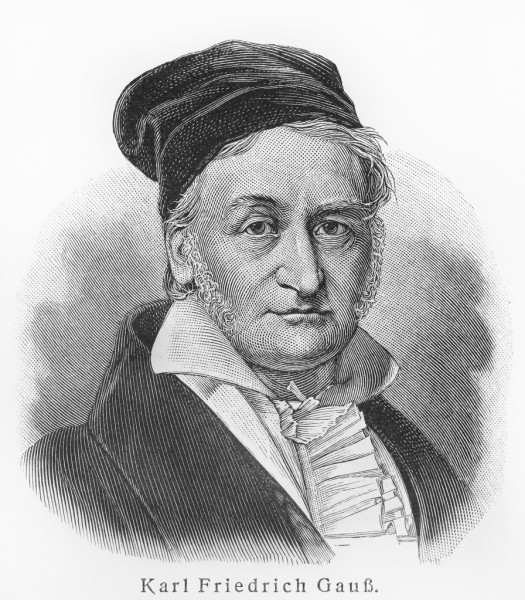
\includegraphics[keepaspectratio,
                     height=0.7\paperheight]{carl-gauss.jpg}
  \end{center}
\end{frame}


\begin{frame}
  \begin{block}{Определение из Википедии}
    \textbf{Машинное обучение} (англ. machine learning, ML) — класс методов искусственного интеллекта, характерной чертой которых является не прямое решение задачи, а обучение за счёт применения решений множества сходных задач.
  \end{block}

  \vspace{1cm}
  Для построения таких методов используются средства математической статистики, численных методов, математического анализа, методов оптимизации, теории вероятностей, теории графов, различные техники работы с данными в цифровой форме.
\end{frame}


\begin{frame}
  \frametitle{Что это?}
  \begin{align*}
  \frac{\partial \rho}{\partial t} + \frac{\partial(\rho u_{i})}{\partial x_{i}} &= 0 \\
  \frac{\partial (\rho u_{i})}{\partial t} + \frac{\partial[\rho u_{i}u_{j}]}{\partial x_{j}} &= -\frac{\partial p}{\partial x_{i}} + \frac{\partial \tau_{ij}}{\partial x_{j}} + \rho f_{i}
  \end{align*}

  \pause
  \vspace{1cm}
  В машинном обучении нет предзаданной модели с уравнениями...
\end{frame}


\begin{frame}
  \frametitle{Два типа обучения}
  \begin{itemize}
    \item Обучение по прецедентам (обучение с учителем), или индуктивное обучение, основано на выявлении эмпирических закономерностей в данных.
    \item Дедуктивное обучение предполагает формализацию знаний экспертов и их перенос в компьютер в виде базы знаний.
  \end{itemize}

  Дедуктивное обучение принято относить к области \textit{экспертных систем}, поэтому \textit{машинное обучение} $\sim$ \textit{обучение по прецедентам}.

  \vspace{0.5cm}
  Многие методы машинного обучения разрабатывались как альтернатива классическим статистическим подходам. Многие методы тесно связаны с извлечением информации (англ. information extraction, information retrieval), интеллектуальным анализом данных (data mining).
\end{frame}


{ % all template changes are local to this group.
    \setbeamertemplate{navigation symbols}{}
    \begin{frame}<article:0>[plain]
        \begin{tikzpicture}[remember picture,overlay]
            \node[at=(current page.center)] {
                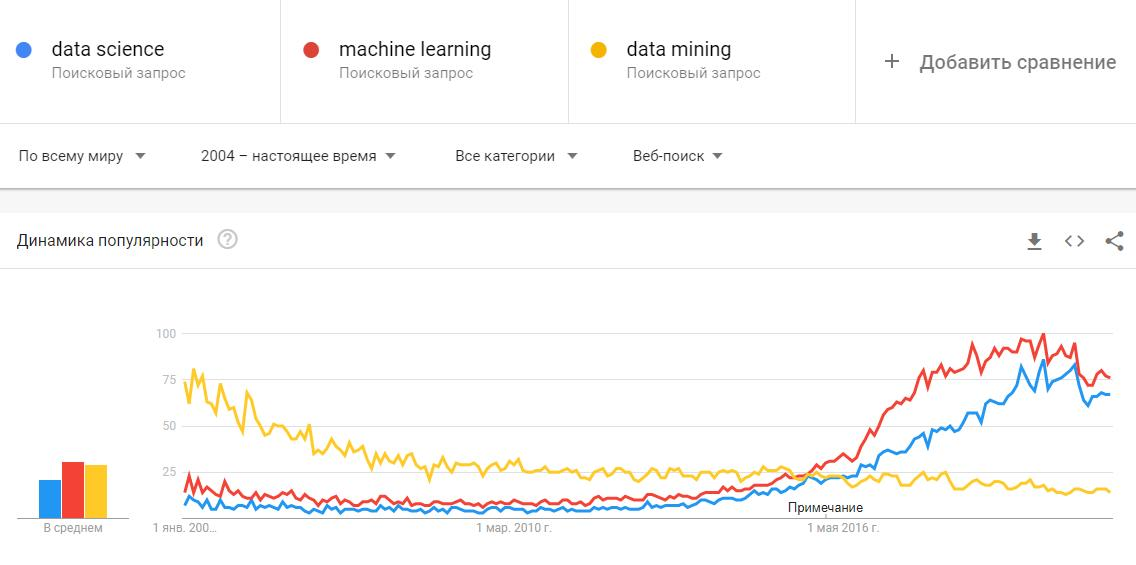
\includegraphics[keepaspectratio,
                                 width=\paperwidth,
                                 height=\paperheight]{ds_ml_google_trends.jpg}
            };
        \end{tikzpicture}
     \end{frame}
}


\begin{frame}
  \frametitle{Математическая постановка}

  $X$ — множество объектов

  $Y$ — множество ответов

  $y: X \to Y$ — неизвестная зависимость (target function)

  \vspace{0.5cm}
  Задача по обучающей выборке (training sample) $\{x_1,\dots,x_\ell\} \subset X$

  с известными ответами $y_i=y(x_i)$

  \vspace{0.5cm}
  найти

  $a: X \to Y$ — алгоритм,

  решающую функцию (decision function), приближающую $y$ на всём множестве $X$
\end{frame}


\begin{frame}
  Всё машинное обучение про это:
  \begin{itemize}
    \item как задаются объекты $x_i$ и какими могут быть ответы $y_i$
    \item в каком смысле «$a$ приближает $y$»
    \item как строить функцию $a$
  \end{itemize}
\end{frame}


\begin{frame}
  \frametitle{Объекты и их признаки}
  $f_j: X \to D_j$

  Вектор $(f_1(x), \dots, f_n(x))$ — признаковое описание объекта $x$

  \vspace{0.5cm}
  Типы признаков:
  \begin{itemize}
    \item $D_j = \{0, 1\}$ — бинарный
    \item $\#|D_j| < \infty $ — категориальный (номинальный)
    \item $\#|D_j| < \infty, D_j$ упорядочено — ординальный (порядковый)
    \item $D_j = \mathbb{R}$ — вещественный (количественный)
  \end{itemize}

  \vspace{0.5cm}
  Матрица «объекты-признаки» (feature data)

  $$F = ||f_j(x_i)||_{\ell\times n} = \left[ {\begin{array}{ccc}
     f_1(x_1) & \dots & f_n(x_1) \\
       \dots  & \dots &   \dots  \\
     f_1(x_\ell) & \dots & f_n(x_\ell)
    \end{array} } \right]$$
\end{frame}


\begin{frame}
  \begin{question}
    Как перевести все признаки в бинарные?
  \end{question}

\end{frame}


\begin{frame}
  \frametitle{Типы задач}

  \begin{block}{Классификация (classification)}
    \begin{itemize}
      \item $Y = \{-1, +1\}$ — бинарная классификация
      \item $Y = \{1, \dots, M\}$ —  многоклассовая классификация
      \item $Y = \{0, 1\}^M$ —  многоклассовая с пересекающимися классами
    \end{itemize}
  \end{block}


  \begin{block}{Регрессия (regression)}
    $Y = \mathbb{R}$ или $Y = \mathbb{R}^m$
  \end{block}

  \begin{block}{Ранжирование (ranking)}
    $Y$ — конечное упорядоченное множество
  \end{block}
\end{frame}


\begin{frame}
  \frametitle{Предсказательная модель}

  Модель (predictive model) — параметрическое семейство функций

  $$A = \{g(x, \theta) | \theta \in \Theta\},$$

  где $g: X \times \Theta \to Y$ — фиксированная функция, $\Theta$ — множество допустимых значений параметра $\theta$

  \begin{block}{Пример}
    Линейная модель с вектором параметров $\theta = (\theta_1, \dots, \theta_n), \Theta = \mathbb{R}^n$:

    $g(x, \theta) = \sum\limits_{j=1}^n \theta_jf_j(x)$ — для регрессии и ранжирования, $Y = \mathbb{R}$

    $g(x, \theta) = \mathrm{sign}\sum\limits_{j=1}^n \theta_jf_j(x)$ — для классификации, $Y = \{-1, +1\}$
  \end{block}
\end{frame}


\begin{frame}
  \begin{block}{Этап обучения (train)}
    Метод $\mu$ по выборке $(X, Y) = (x_i, y_i)_{i=1}^\ell$ строит алгоритм $a = \mu(X, Y)$

    $$
    \boxed{
    \left[ {\begin{array}{ccc}
       f_1(x_1) & \dots & f_n(x_1) \\
         \dots  & \dots &   \dots  \\
       f_1(x_\ell) & \dots & f_n(x_\ell)
      \end{array} } \right]
    \xrightarrow{y}
    \left[ {\begin{array}{c}
    y_1 \\ \dots \\ y_\ell \end{array} }\right]
    \thinspace}
    \xrightarrow{\mu} a
    $$
  \end{block}

  \begin{block}{Этап применения (test)}
    Алгоритм $a$ для новых объектов $x_i^\prime$ выдаёт ответы $a(x_i^\prime)$
  \end{block}
\end{frame}


\begin{frame}
  \frametitle{Функционалы качества}

  $\mathcal{L}(a, x)$ — функция потерь (loss function). Величина ошибки алгоритма $a \in A$ на объекте $x \in X$.

  \begin{block}{Функции потерь для задач классификации}
    $\mathcal{L}(a, x) = [a(x)\neq y(x)]$  —  индикатор ошибки
  \end{block}

  \begin{block}{Функции потерь для задач регрессии}
    \begin{itemize}
      \item $\mathcal{L}(a, x) = |a(x) - y(x)|$ — абсолютное значение ошибки
      \item $\mathcal{L}(a, x) = (a(x) - y(x))^2$ — квадратичная ошибка
    \end{itemize}

  \end{block}

  \textit{Эмпирический риск} – функционал качества алгоритма $a$ на $X^\ell$:
  $$Q(a, X^\ell) = \frac{1}{\ell} \sum\limits_{i=1}^\ell \mathcal{L}(a, x_i)$$
\end{frame}


\begin{frame}{Сведение задачи обучения к задаче оптимизации}

  Метод минимизации эмпирического риска

  $$\mu(X^\ell) = \arg\min\limits_{a \in A} Q(a, X^\ell)$$

  \begin{block}{Пример}
    Метод наименьших квадратов: ($Y = \mathbb{R}, \mathcal{L}$ квадратична)

    $$\mu(X^\ell) = \arg\min\limits_{\theta} \sum\limits_{i=1}^{\ell} (g(x_i, \theta) - y_i)^2$$
  \end{block}


  \begin{block}{Проблема обобщающей способности}
    \begin{itemize}
      \item Найдём ли мы «закон природы» или переобучимся, то есть подгоним функцию $g(x_i, \theta)$ под заданные точки?
      \item Будет ли $a = \mu(X^\ell)$ приближать функцию $y$ на всём $X$?
      \item Будет ли $Q(a, X^k)$ мало на новых данных — контрольной выборке $X^k = (x_i^\prime, y_i^\prime)_{i=1}^k$, $y_i^\prime = y(x_i)$?
    \end{itemize}
  \end{block}

\end{frame}

\begin{frame}
  \frametitle{Демо: пример переобучения}

  \href{https://github.com/avalur/yandex-practice-2022/blob/main/01_intro/01_demo_overfitting.ipynb}{Разбираемся с кодом!}
\end{frame}


\begin{frame}{Переобучение}
  \framesubtitle{одна из главных проблем в машинном обучении}

  \begin{block}{Из-за чего возникает переобучение?}
    \begin{itemize}
      \item избыточная сложность пространства параметров $\Theta$, лишние степени свободы в модели $g(x, \theta)$ «тратятся» на чрезмерно точную подгонку под обучающую выборку
      \item переобучение есть всегда, когда есть оптимизация параметров по конечной (заведомо неполной) выборке
    \end{itemize}
  \end{block}

  \begin{block}{Как обнаружить переобучение?}
    Эмпирически, путём разбиения выборки на train и test
  \end{block}

  \begin{block}{Нельзя избавиться от него совсем. Как минимизировать?}
    \begin{itemize}
      \item минимизировать ошибку на валидации (HoldOut, Leave One Out, Cross Validation), но осторожно!
      \item накладывать ограничения на $\theta$ (регуляризация)
      \item минимизировать одну из теоретических оценок
    \end{itemize}
  \end{block}
\end{frame}


\begin{frame}{Эмпирические оценки обобщающей способности}
  \begin{itemize}
    \item Эмпирический риск на тестовых данных (hold-out)

      $$HO(\mu, X^\ell, X^k) = Q(\mu(X^\ell), X^k) \to \min$$

    \item Скользящий контроль (leave-one-out), $L = \ell + 1$

      $$LOO(\mu, X^\ell) = \frac1L \sum\limits_{i=1}^L \mathcal{L}(\mu(X^\ell\backslash \{x_i\}), x_i) \to \min$$

    \item Кросс-проверка (cross-validation), $L = \ell + k, X^L = X^\ell_n \cup X^k_n$:

      $$CV(\mu, X^L) = \frac1{|N|} \sum\limits_{n \in N} {Q}(\mu(X^\ell_n), X^k_n) \to \min$$
  \end{itemize}
\end{frame}

{ % all template changes are local to this group.
    \setbeamertemplate{navigation symbols}{}
    \begin{frame}<article:0>[plain]
        \begin{tikzpicture}[remember picture,overlay]
            \node[at=(current page.center)] {
                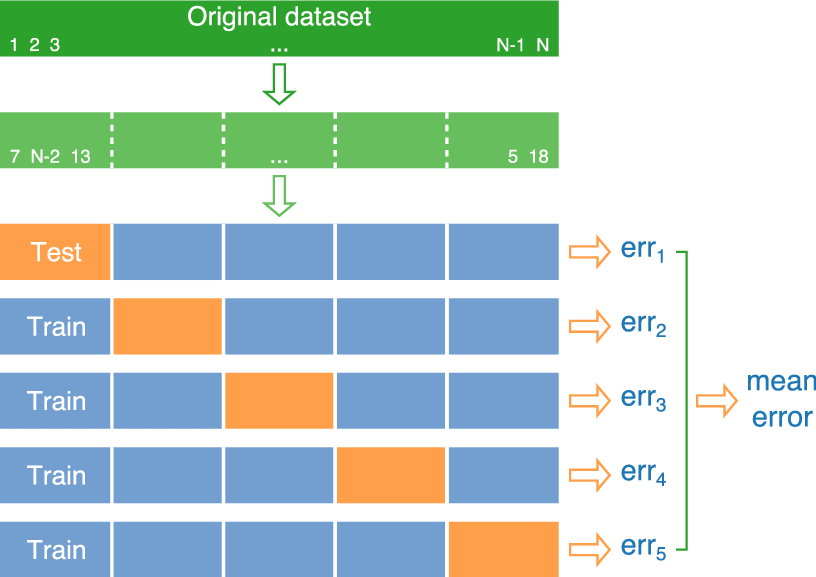
\includegraphics[keepaspectratio,
                                 width=\paperwidth,
                                 height=\paperheight]{A-schematic-illustration-of-K-fold-cross-validation-for-K-5-Original-dataset.png}
            };
        \end{tikzpicture}
     \end{frame}
}

\begin{frame}{Ключевые события в машинном обучении}
  \begin{itemize}
    \item[1997] IBM Deep Blue обыгрывает чемпиона мира по шахматам Гарри Каспарова
       \begin{itemize}
         \item 480 шахматных CPU
         \item перебор модификацией альфа-бета-отсечений
         \item две дебютные книги
       \end{itemize}

      \pause
      \item[2004] Соревнование беспилотных автомобилей: DARPA Grand Challenge
         \begin{itemize}
           \item призовой фонд \$1 млн
           \item в первом заезде победитель проехал 11.8 из 230 км
         \end{itemize}

      \pause
      \item[2006] Запуск Google Translate
         \begin{itemize}
           \item сначала статистический машинный перевод
           \item мобильное приложение появилось в 2010
         \end{itemize}
  \end{itemize}
\end{frame}


\begin{frame}
  \begin{itemize}
    \item[2011] 40 лет развития DARPA CALO (Cognitive Assistant that Learns and Organizes)
       \begin{itemize}
         \item появление голосового помощника Apple Siri
         \item IBM Watson победил в телевизионной игре «Jeopardy!» (у нас «Своя игра»)
       \end{itemize}

       \pause
       \item[2011-15] ImageNet: 25\% -> 3.5\% ошибок против 5\% у людей

       \pause
       \item[2015] Создание открытой компании OpenAI, Илон Маск и Сэм Альтман, обещали вложить \$1 млрд

       \pause
       \item[2016] Google DeepMind AlphaGo обыграл чемпиона мира по игре Го

       \pause
       \item[2018] На аукционе Christie's картина, формально нарисованная ИИ, продана за 432 500\$

       \pause
       \item[2020] AlphaFold 2 предсказывает структуру белков с точностью выше 90\% для примерно двух третей белков в датасете
  \end{itemize}

\end{frame}

\begin{frame}
  \frametitle{Резюме}
  \begin{itemize}
    \item Основные понятия машинного обучения:

    обучение по прецендентам (с учителем),

    объекты, признаки, ответы, модель алгоритмов, метод обучения, эмпирический риск, переобучение

    \item Проблема переобучения: HoldOut, LeaveOneOut, CrossValidation

    \item Ключевые события в машинном обучении
  \end{itemize}
\end{frame}

\end{document}
